In order to evaluate the approach proposed in this paper, we have collected
a dataset with a car in an urban setting. Our car is equipped with a Sony
XCD-SX910 camera recording $1280$x$960$ images at $3.75$ frames per second and
an XSens MTi IMU running at $100$ Hz with $x$ pointing forward, $y$ to the
right, and $z$ upward. The sequence contains $8218$ images and lasts around $40$
minutes. We have encountered different scenes comprising of traffic lights,
crosswalks, or changes of speed limit. We have driven in a loop so as to come
several times in the same situation and thus have an estimation of the quality
of our solution.

In the rest of this Section, we first display an experiment of the whole
algorithm on synthetic data. It is easier to have a ground truth on simulated
data and hence validate our approach. We then show results on real-world data
with a detailed analysis of all the components.

\subsection{Simulation}
For visualization purposes, we have simulated IMU data with an univariate normal
distribution and have introduced change-points every $50$ data points. We have
randomly generated 3 different $\boldsymbol{\alpha}_i$ with $K=256$ coding for
the traffic situations.

Fig.~\ref{fig:simulation} depicts the output of the simulation and demonstrates
the pertinence of our method. The code runs in MATLAB with no attempt for
optimization and has a processing time of about $0.3$ seconds per time step. In
a realistic scenario, histogram building from image adds up to the time.

\begin{figure}[t]
\centering
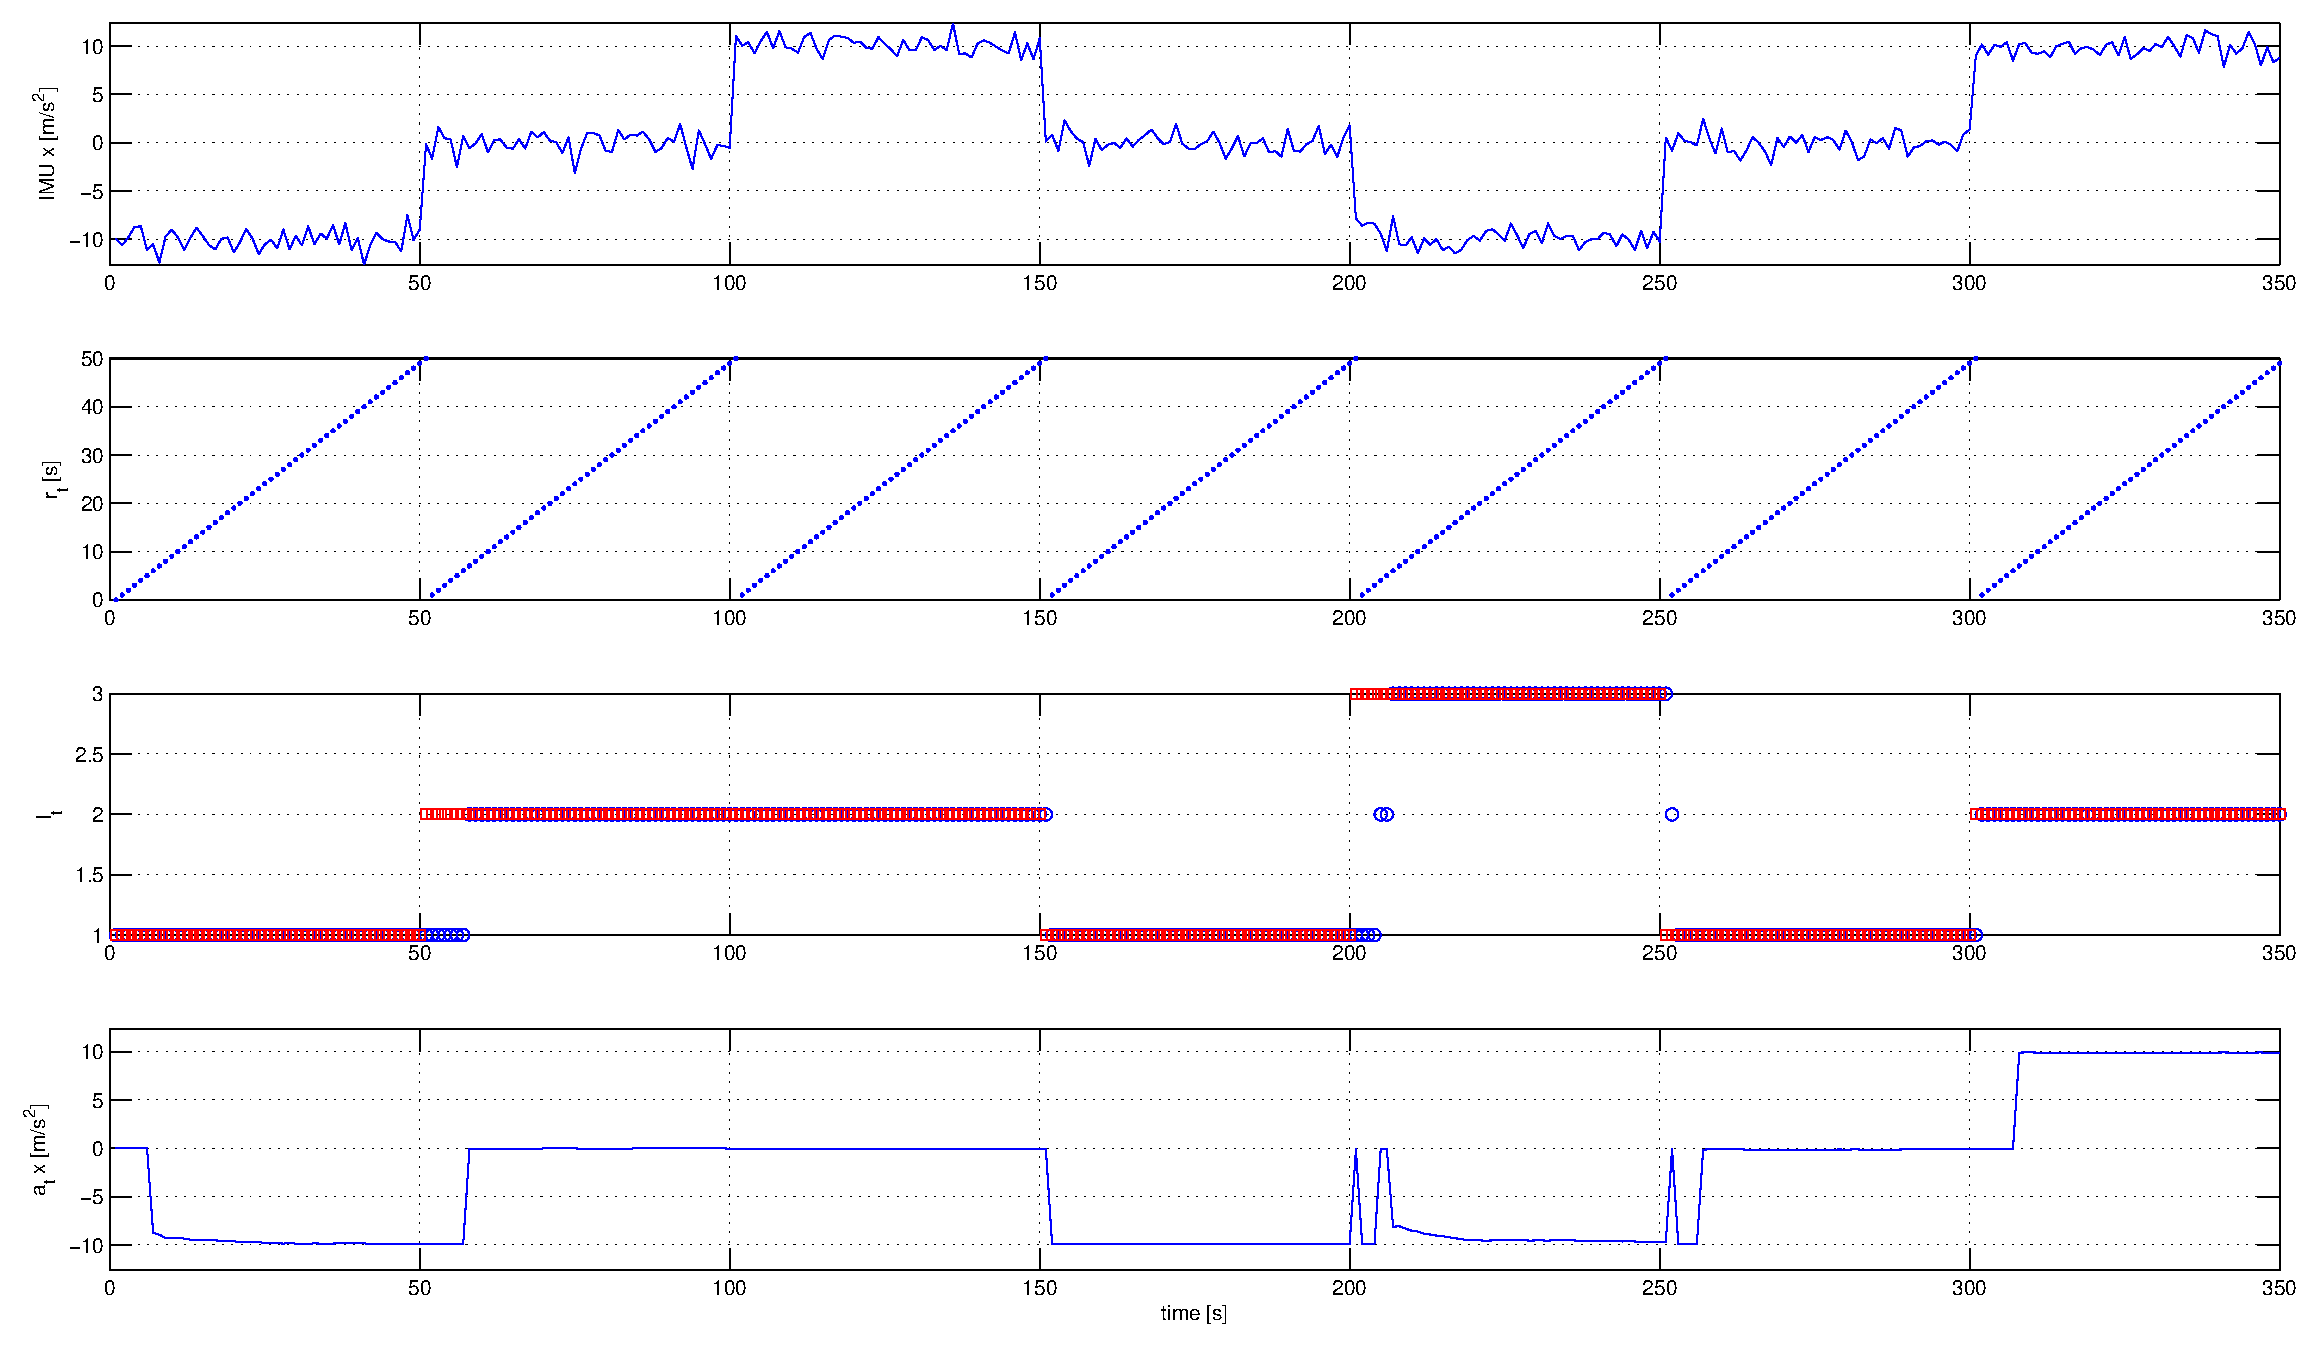
\includegraphics[width=\columnwidth]{fig/simResult.eps}
\caption{Simulation results of the entire algorithm. From top to bottom, the
plots display the simulated IMU data $\mathbf{z}_t$, the inferred segment
lengths $r_t$, the inferred labels $l_t$ (blue circle) and ground truth
(red square), the MAP for $\mathbf{a}_t$.}
\label{fig:simulation}
\end{figure}

\subsection{Motion Segmentation}
In this experiment, we want to estimate the quality of our motion segmentation
algorithm from Section~\ref{sec:motion}. We performed inference on the
final posterior distribution $p(r_t\mid \mathbf{z}_{1:t})$ to get the optimal
sequence of segment lengths which represents our motion segments. We set the
hazard rate to $\lambda=1/10$, the number of particles to $P=100$, and the prior
hyperparameters of the normal-Wishart to $\kappa_0=1,
\boldsymbol{\rho}_0=\mathbf{0},\nu_0=3,\boldsymbol{\Lambda}_0=\mathbf{I}$. We
only considered IMU data at $10$ Hz.

Fig.~\ref{fig:motion_segments} shows the extracted motion segments along with
the corresponding IMU data. Our algorithm identified $165$ segments which are
validated by visual inspection of the IMU data. Furthermore, the segmentation
has been compared to a manual annotation of our image sequence and exhibited an
accuracy of approximatively $92\%$. For the labeling of the change-points, we
have watched the video and noted down where we would expect a change of driving
behavior. The parameter $\lambda$ controls the false positives/negatives rates.
As expected, the typical motion patterns that appeared were driving straight
with no acceleration, driving straight with acceleration or deceleration, and
turning left or right.

\begin{figure}[t]
\centering
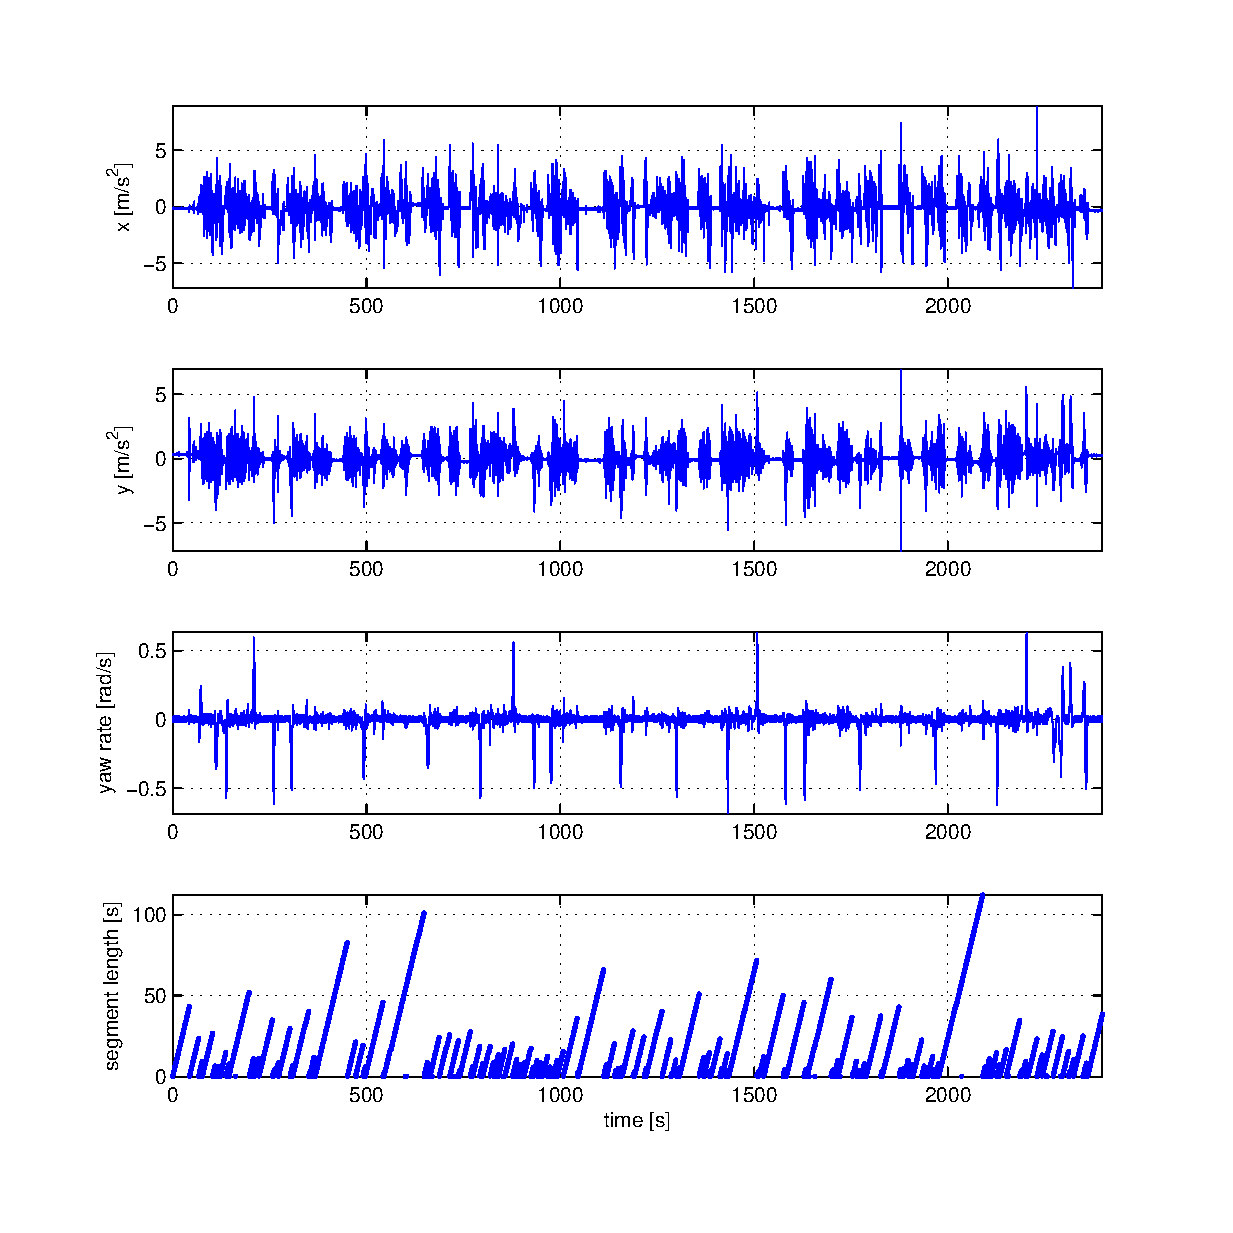
\includegraphics[width=\columnwidth]{fig/cpResult.eps}
\caption{Optimal motion segmentation from IMU data. The three top plots are the
IMU raw values over time. The bottom plot depicts the motion segments
discovered by our algorithm.}
\label{fig:motion_segments}
\end{figure}

\subsection{Traffic Situation Labeling and Recognition}
In this second experiment, we are interested in evaluating the part of our
algorithm presented in Sec.~\ref{sec:labeling}. We want to see how many traffic
situations models were discovered and what they represent. Moreover, we want
to see if we can re-associate place models in other runs at the same place.

SIFT descriptors have been computed on a grid of $l=8$x$8$. We have created a
dictionary of $K=1024$ SIFT features from $N=400$ images randomly picked in our
dataset. The pyramid representations were generated on $L=3$ levels. The prior
of the DCM for a new motion segment was learned from the same $N$ images. The
probability for a new label was set to $p_{new}=0.5$ and the Chi-square
threshold to $\xi=0.1$.
